\chapter{Requirement and Analysis}
\section{Introduction}
The overall purposes of this project is to create a system to improve efficiencies of \gls{ic}'s digital document management strategies. 
The study involves investigating internal \gls{ic}'s working procedures and regulations.
How \gls{ic} execute strategies on their digital document assets.
What are advantages and disadvantages of their strategies.
Gaining such information is valuable to this study because plausible solutions could be proposed and implemented. 
Solutions that could further improve flows of documents inside \gls{ic}.
This chapter presents requirement gathering methods to address the problem.

\section{Gathering Requirements}
To understand what user expects the system to do is an essential part of developing a software.
The more system operates close to their expectation, the more satisfaction they get.
User's expectation on the system can be described as requirements.
A descriptive text describes the system's functionality.
What they are and why the user need them.
The following sections discuss these two strategies in order to gather requirements from the user.

\subsection{Interview}
\citeauthor{gall7j} (\citeyear{gall7j}) states that interview is the spontaneous generation of questions in a natural interaction, typically one that occurs as part of ongoing participant observation fieldwork.
\citeauthor{brady2011craft} (\citeyear{brady2011craft}) points out that what interviewer and salesman have in common is potential customers whom one could hold their attention to talk.
Getting an interview means making an appointment to see the subject, identifying questions related to the research topic, and showing on time for the interview.
The purpose of interview is to gain information from interviewee by having interviewer asking questions.
Researchers can gain useful insights from the subject who is expertise in one's field.

Figure \ref{ic-org-sturcture} shows \gls{ic}'s organization structure.
The top-most is the dean followed by deputy dean then assistant of deputy dean.
On the right hand side are committee members.
Only academic and academic support located at the bottom-most hierarchy involves archiving documents.
 \begin{figure}[h]
 	\centering
 	\caption{\gls{ic} organization's structure}
 	\label{ic-org-sturcture}
 	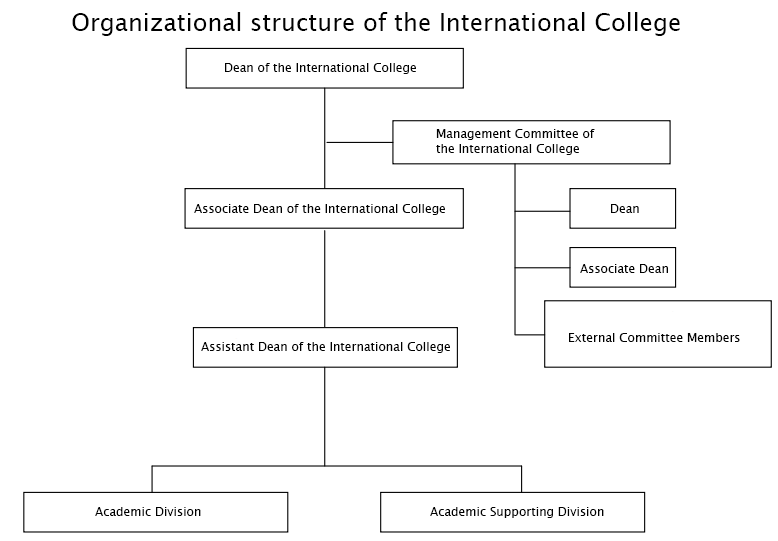
\includegraphics[scale=0.7]{res/requirement/ic-org}
 \end{figure}

In this study, \gls{ic} staffs are the subject of this study divided into two focus groups:
\begin{description}
	\item [Academic staffs] as a primary focus group because they are responsible for keeping records of all \gls{ic}'s documents.
	Transfer documents around the organization according to \gls{ic}'s workflow specifications.
	Managing day-to-day operations within the organization.
	They also provide academic advices and guidances to \gls{ic} undergraduate and postgraduate students.

	\item [Administrative staffs] as a secondary focus group because they are directly involve in keeping and organizing documents.
	Some of them have privilege to issue, review, and approve documents.
	In order to know more about their procedures, deputy dean and deputy dean's assistant are selected as a sample for this study.
\end{description}

After conducting the questionaire interview, \gls{ic} staffs reveal that they would like a system that manage their organization's documents automatically.
What they mean by managing is that they would like to know what are they suppose to do with received documents.
Things they have to do could be approval, signing, or printing documents.
Then, forwarding the document to another person who is involved in the workflow. 
They also would like to know any additional documents required before forwarding documents so that they can prepare them beforehand.

For every official \gls{ic}'s documents, \gls{ic} assigns an identification number internally.
There are eleven types of documents separated into three categories based on head of the department who is responsible for those documents as shown in table \ref{tbl-doc-subtype}.
\begin{table}[h]
	\caption{Document type with identification code separated by category}
	\label{tbl-doc-subtype}
	\centering
\begin{tabular}{llC{3cm}}
	\hline
	Category & Document Type & Identification Code \\
	\hline
	General Management 1 & Archive & AA \\
	& Human Resources & AB \\
	& Quality Assurance & AC \\
	& Parcel & AD \\
	& IT/KM & AE \\
	\midrule
	General Management 2 & Plan and Risk Management & BA \\
	& Accounting & BB \\
    & Research & BC \\
	& Academic Management & BD \\
	\midrule
	Academic & Academic Administration & CA \\
	& Student Affairs & CB \\
	\hline
\end{tabular}
\end{table}

According to the scope stated in section \ref{sec:scope}, each document form has its own document type as can be seen in table \ref{tbl-scope-doc-subtype}.
External documents are not \gls{ic}'s official documents in table \ref{tbl-doc-subtype}.
They are attachments of the official document.
\begin{table}
	\centering
	\caption{Association between document stated in \ref{sec:scope} and document type in table \ref{tbl-doc-subtype}}
	\label{tbl-scope-doc-subtype}
\begin{tabular}{ll}
	Document Form & Document Type \\
	\hline
	Absence Form & Academic Administration \\
	Student Internship Form & Student Affairs \\
	Conference Outside \gls{kmitl} Form & Academic Administration \\
	\hline
\end{tabular}
\end{table}

To generate an identification number for a document, it has to confine to the following format: $TTYYYYDDDD$.
Where $TT$ is the identification code from table \ref{tbl-doc-subtype}.
$YYYY$ is a four-digit such as 2016 or 2015.
$DDDD$ is a four-digit running number.
It starts at one and must increment by one each time as the new document is created.
If $DDDD$ is less than one thousand, it must fill with leading zeros until there are four digits presents.
If the number is greater than 9999 which is a maximum limit, it has to continue counting normally but without any leading zeros.
Although, having the same type of document more than ten thousand documents has never happened to \gls{ic} before.
If new year has started, the $DDDD$ must reset back to one (0001).

To clarify how the identification number is generated and combined together, assume that \gls{ic} already have two documents of type \enquote{Academic Administration}(CA).
Mr. X would like to take a vacation on May, 2016.
So he requests an \enquote{Absence Form} and put in an information.
Then, he submits the form to the system.
The absence form is a part of academic administration so $TT$ is \enquote{CA}.
The document is created at 2016 so $YYYY$ is \enquote{2016}.
Because there are two documents already in the system.
The next number is three so $DDDD$ is \enquote{0003}.
Combining $TT$, $YYYY$, and $DDDD$ together yields CA20160003.

\subsection{Case Study}
The figure \ref{fig:our-case-study-method} shows a case study of \gls{ic}'s documents in 2015.
The case study is divided into three cases:
\begin{enumerate*}
	\item storing digital documents;
	\item retrieving digital documents;
	\item tracking digital documents.
\end{enumerate*}
Each case comprises of four types of documents;
\begin{enumerate*}
	\item absence form;
	\item student internship form;
	\item conference outside \gls{kmitl} form;
	\item external document.
\end{enumerate*}
They come from the scope stated in section \ref{sec:scope}.

\begin{figure}[h!]
	\centering
	\caption{Case study of this project}
	\label{fig:our-case-study-method}
	\begin{minipage}{8cm}\dirtree{%
		.1 Documents.
		.2 \gls{ic}'s Documents Observed in 2015.
		.3 Storing Digital Documents.
		.4 Absence Form.
		.4 Student Internship Form.
		.4 Conference Outside \gls{kmitl} Form.
		.4 External Digital Documents.
		.3 Retrieving Digital Documents.
		.4 Absence Form.
		.4 Student Internship Form.
		.4 Conference Outside \gls{kmitl} Form.
		.4 External Digital Documents.
		.3 Tracking Digital Documents.
		.4 Absence Form.
		.4 Student Internship Form.
		.4 Conference Outside \gls{kmitl} Form.
		.4 External Digital Documents.
		}
	\end{minipage}
\end{figure}

These mentioned forms emerge from a specific type of \gls{ic}'s official documents.
External digital documents are unofficial documents because \gls{ic} isn't the one who issue the documents.
Thus, figure \ref{fig:our-case-study-method} can be rewritten for simplicity as shown in figure \ref{fig:our-case-study-method-rewrite}.
\begin{figure}[h!]
	\centering
	\caption{Simpler version of figure \ref{fig:our-case-study-method}}
	\label{fig:our-case-study-method-rewrite}
	\begin{minipage}{8cm}\dirtree{%
			.1 Documents.
			.2 \gls{ic}'s Documents Observed in 2015.
			.3 Storing Digital Documents.
			.4 Official Documents.
			.4 Unofficial Documents.
			.3 Retrieving Digital Documents.
			.4 Official Documents.
			.4 Unofficial Documents.
			.3 Tracking Digital Documents.
			.4 Official Documents.
			.4 Unofficial Documents.
		}
	\end{minipage}
\end{figure}

The workflow of each type of forms are represented as an activity digram shown in figure \ref{fig:diagram-absence}, \ref{fig:diagram-student-internship}, and \ref{fig:diagram-conference}.
The common operation that appears on all diagram is that someone has to either approve or reject the document.
User is the person who initiate the document, filling forms, and submit to the staff for approval.
\enquote{Absence form} and \enquote{Conference outside \gls{kmitl} form} requires user, staff, and dean to sign the document.
If someone reject the document, user has to be notified about the rejection.
The final process is to \enquote{finalize document} as shown in figure \ref{fig:diagram-finalize-document}.
Staff has to upload attachments as an evidence acquired from scanning to the system. 
Then, the system will notify user that the submitted document has completed successfully.
\begin{figure}[h]
	\centering
	\caption{An activity diagram for \enquote{Absence form}}
	\label{fig:diagram-absence}
	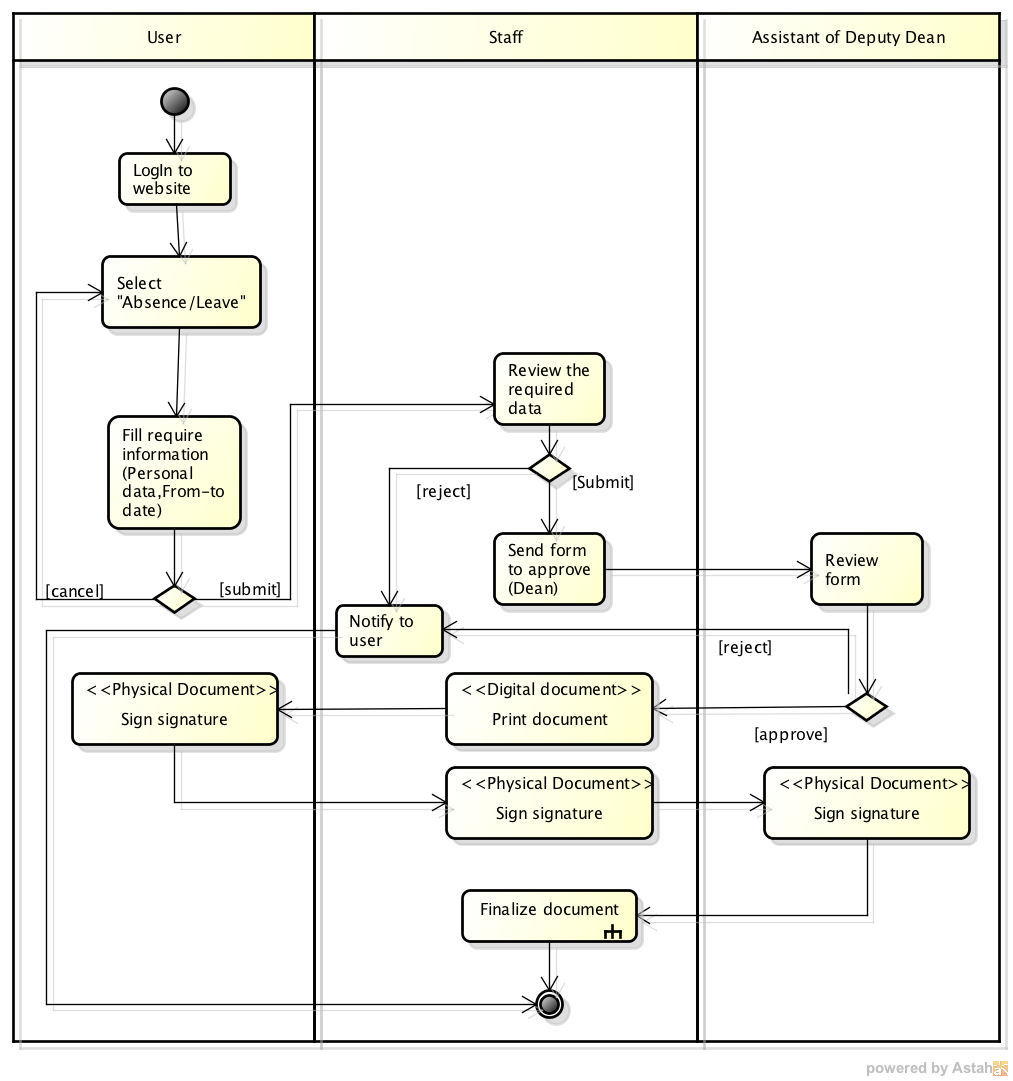
\includegraphics[scale=0.5]{res/requirement/absence}
\end{figure}

\begin{figure}
	\centering
	\caption{An activity diagram for \enquote{Student internship form}}
	\label{fig:diagram-student-internship}
	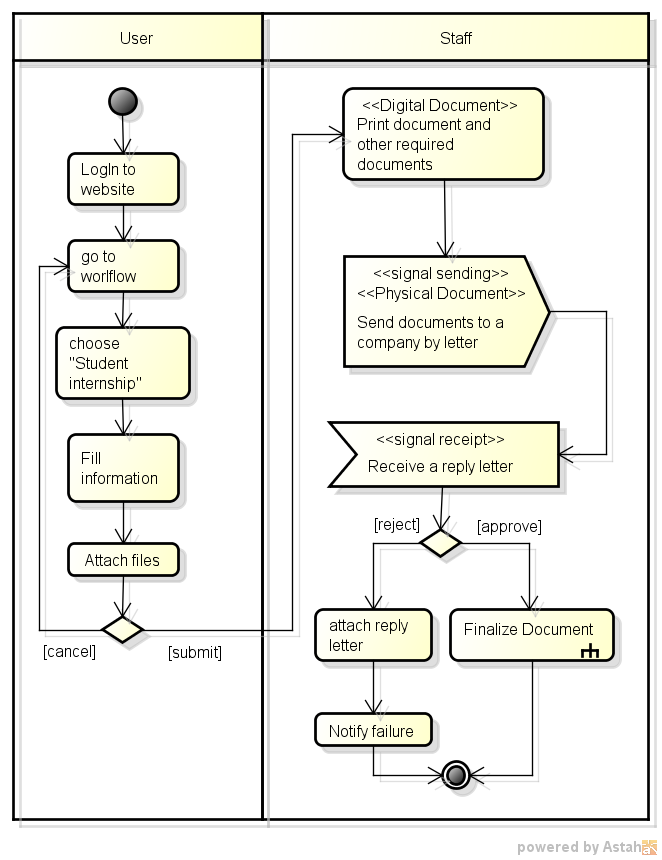
\includegraphics[scale=0.7]{res/requirement/student_internship}
\end{figure}

\begin{figure}
	\centering
	\caption{An activity diagram for \enquote{Conference outside \gls{kmitl} form}}
	\label{fig:diagram-conference}
	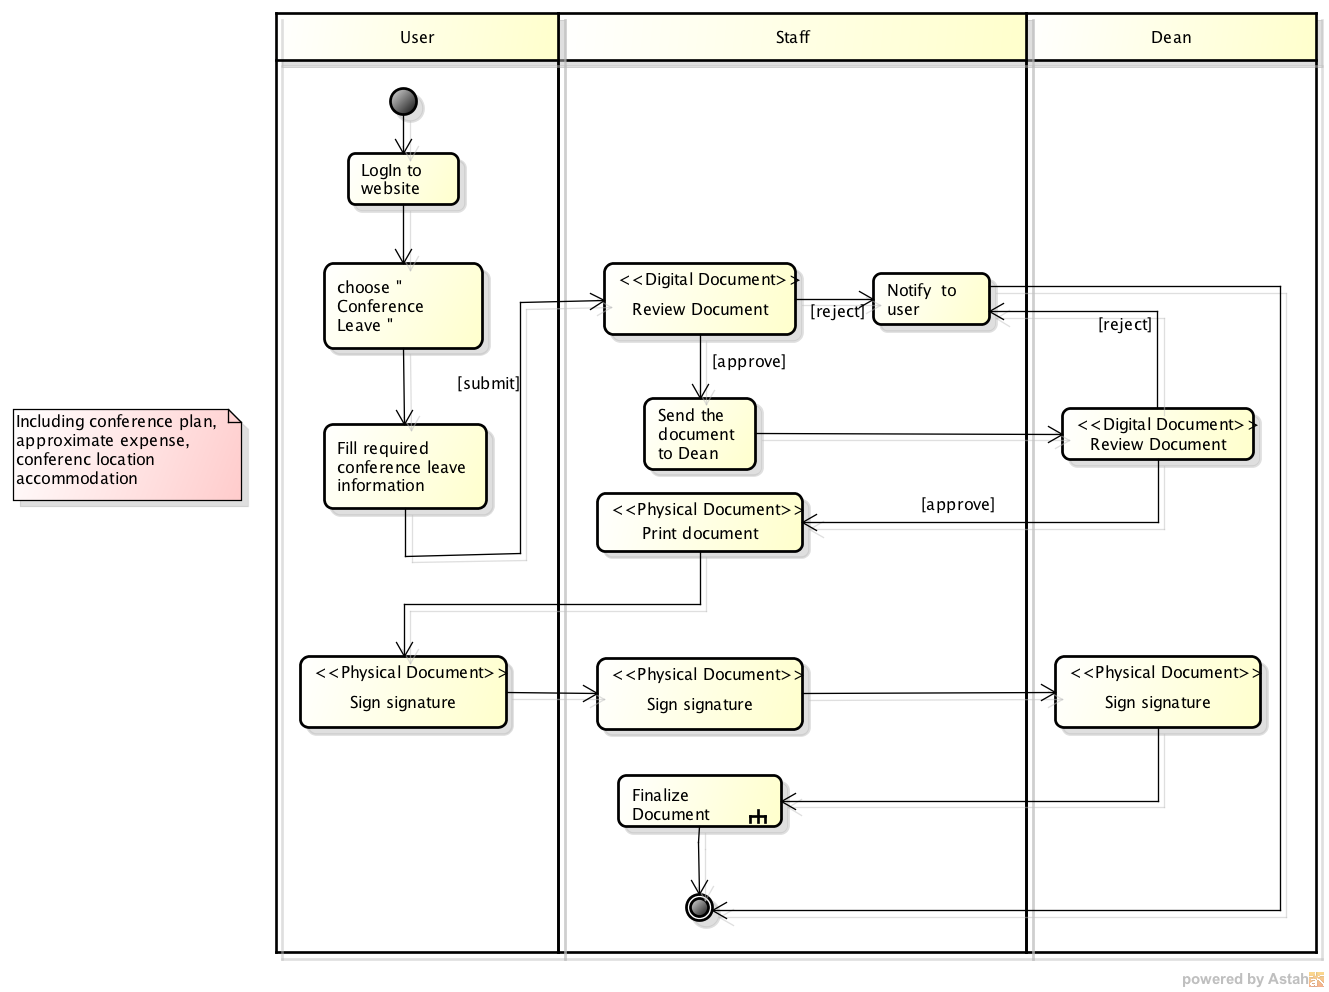
\includegraphics[scale=0.45]{res/requirement/conference}
\end{figure}

\begin{figure}
	\centering
	\caption{A sub activity diagram of task \enquote{Finalize document}}
	\label{fig:diagram-finalize-document}
	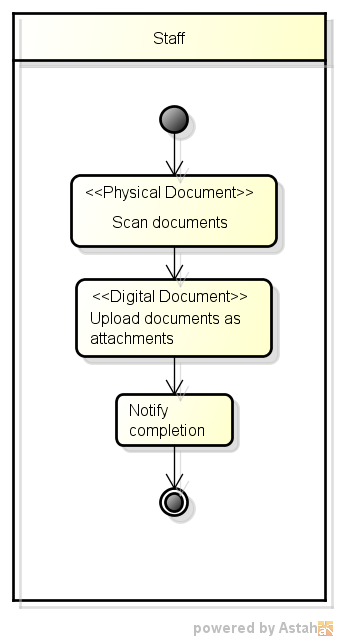
\includegraphics[scale=0.5]{res/requirement/finalize_document}
\end{figure}

\section{Requirement Summary}
This section summarizes software requirements into itemized lists.
There are two subsections, user requirement and system requirement.

\subsection{User Requirement}
User requirement is a goal or task that specific classes of users must be able to perform with a system, or a desired product attribute \cite{wiegers_2003}.
\begin{enumerate}
	\item 
	User shall be able to includes digital attachment files to the document as it states.
	
	\item
	Staff including dean shall be able to read documents.
	Then perform either the following actions: reject or approve the document.
	
	\item
	Staff shall be able to print out paper documents from digital documents including attachments.
	
	\item
	If any official document requires physical signature(s) as a conclusive evidence, staff shall be able to scan and upload that document as an attachment of the official document.
	
	\item
	Any \gls{ic} personnel who have a write-access to official documents shall have read-access to all previous versions of those documents.
	
	\item
	User shall be able to search their documents by the following criteria:
	\subitem A document identification code given by the system.
	\subitem A Form's name.
	\subitem A date when the document is created/modified.
	\subitem A Document's status indicates whether the document is rejected, pending, or completed successfully.
	
	Any mentioned criteria can be mixed together to create more complex search queries.
	
	\item
	\label{notification-method}
	User should be notified when their documents are rejected or completed successfully.
	The notification only happens inside the system.
	Meaning that user require to access the system in order to get notified.
	The system notify user by updating document's status to a new one.
	
	\item
	Staff and dean should be notified when there is a new pending document forwarded to them.
	The notification method is the same as \ref{notification-method}.
\end{enumerate}

\subsection{System Requirement}
System requirement is a top-level requirement for a product that contains multiple subsystems, which could be all software or software and hardware \cite{wiegers_2003}.
\begin{enumerate}
	\item The system shall operate as a web application hosted on a web server so that all users can access it in one place.
	\item The system shall not disclose internal workflow to any user for all associated documents except for an administrator.
	\item The system shall assign an identification code to official documents in the format $TTYYYYDDDD$.
	\item The system shall contain the REST \gls{api} so that it can communicate with front-end of this system.
	The \gls{api} shall not be publicly available.
	The \gls{api} shall be in URI \enquote{/api/document/\textless interface \textgreater/} where \textless interface \textgreater is the name of the interface.
	URI, input parameter, output, and description are shown in table \ref{tbl:dms-api}.
\end{enumerate}

\begin{table}[h]
	\caption{A list of \gls{api} of this system}
	\label{tbl:dms-api}
	\begin{tabular}{lcL{3.5cm}L{3.5cm}}
		\hline
		URI & Parameter(s) & Return Value (JSON) & Description \\
		\hline
		
		/api/document/read & User ID, Document ID & A document's metadata on a given ID. & Query a document. \\
		
		/api/document/ref & User ID, Document ID & All previous version of the document & Query all previous version of the document on a given ID. \\
		 
		/api/document/attach & User ID, Document ID & Document's attachments & Query all document's attachment files on a given ID. \\
		
		/api/document/attach & User ID & Document's attachments & Query all user's attachment files in all user's documents. \\
		
		/api/document/delete & User ID, Document ID & \gls{http} response & Delete user's document on a given ID.
		The system must not delete other documents owned by a different user. \\
		\hline
	\end{tabular}
\end{table}


\subsection{Quality Attribute}
Quality attribute is a kind of non-functional requirement that describes a service or performance characteristic of a product \cite{wiegers_2003}.
\begin{enumerate}
	\item The system shall encrypt all documents and attachment files.
	\item The system shall use HTTPS communication protocol to exchange data between a web server and a client.
	\item A user interface should have an English localization available.
	\item A user interface should be intuitive enough that user don't have to rely on a user manual.
	Meaning that user doesn't have to go through many processes to achieve their tasks.
	Big buttons and large self-explanatory texts are also preferable.
\end{enumerate}

\clearpage

\section{Use Case}
\label{section:usecase}
Figure \ref{fig:usecase-diagram} captures system functionalities and requirements represented as \gls{uml} use case diagram.
Table \ref{tbl:actor-description} describes who these type of users are.
From table \ref{tbl:usecase-first} to table \ref{tbl:usecase-last} elaborates each use cases in greater detail.

\begin{figure*}
	\centering
	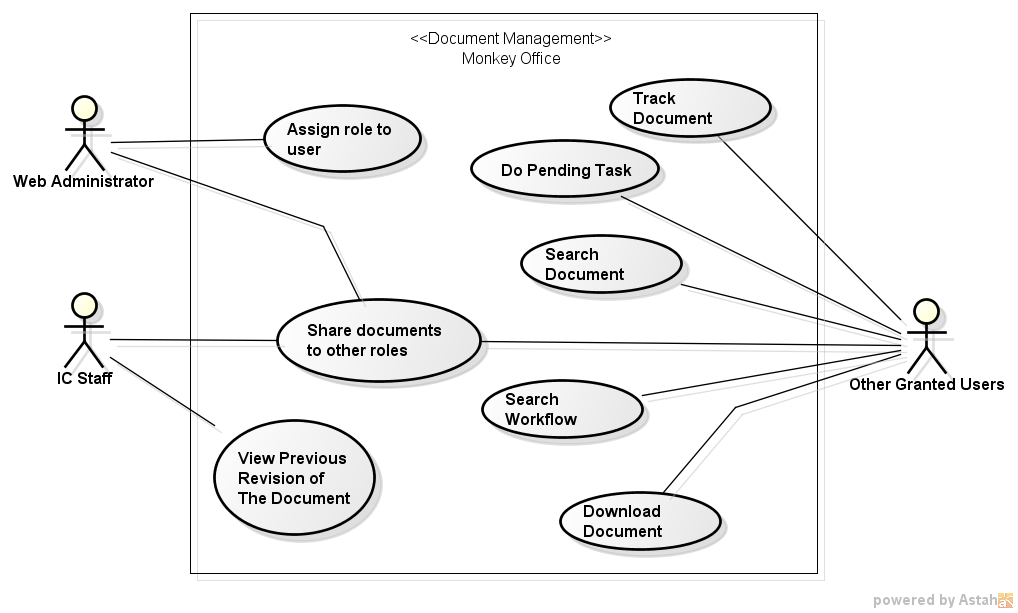
\includegraphics[scale=0.6]{res/software-design/usecase_diagram}
	\caption{A usecase diagram for Monkey Office}
	\label{fig:usecase-diagram}
\end{figure*}

\begin{table}
	\centering
	\caption{Type of user and description}
	\label{tbl:actor-description}
	\begin{tabular}{|l|L{7.5cm}|}
		\hline
		Actor & Description \\
		\hline
		Dean & A headmaster of \gls{ic}. \\
		Deputy dean & Dean's assistant who could also be a dean's representative. \\
		Assistant of deputy dean & Deputy dean's assistant who deals with documents that is not critical to \gls{ic}. \\
		Staff & \gls{ic}'s employee in academic department (refer to bottom-most hierarchy in figure \ref{ic-org-sturcture}) \\
		User & A regular user who have an account provided by an administrator to access the system. \\
		\hline
	\end{tabular}
\end{table}

\newcommand{\alreadylogin}{Have already logged in to the system}
\newcommand{\allICPersonel}{
	\begin{itemize}
		\item Dean
		\item Deputy dean
		\item Assistant of deputy dean
		\item Staff
	\end{itemize}
}

\begin{table}
	\centering
	\caption{Use case: Assign role to user}
	\label{tbl:usecase-first}
	\begin{tabular}{|l|L{9cm}|}
		\hline
		\textbf{Use Case Name} & Assign role to user \\
		\hline
		
		\textbf{Description} & Assigning roles of \gls{ic} such as student or staff to the user. \\
		\textbf{Primary Actor} & Web administrator \\
		\textbf{Pre-condition} & 
		\begin{enumerate}
			\item \alreadylogin.
			\item There is at least one user registers to the system.
		\end{enumerate} \\
		\textbf{Post-condition} & The system assigns a role to user and notify him/her. \\
		\textbf{Trigger} & 
		\begin{enumerate}
			\item A user has registered to the system.
			\item A user request web administrator to change a role.
		\end{enumerate}\\
		\textbf{Basic flow} & 
		\begin{enumerate}
			\item On the top menu-bar, click on the \enquote{Admin} tab.
			\item Navigate to \enquote{Settings} and click on the \enquote{Role Management}
			\item Click on the desired role and select which user to be assigned to.
			\item Click \enquote{save} button.
		\end{enumerate} \\
		\hline
	\end{tabular}
\end{table}

\begin{table}
	\centering
	\caption{Use case: Share documents to other roles}
	\begin{tabular}{|l|L{9cm}|}
		\hline
		\textbf{Use Case Name} & Share documents to other roles \\
		\hline
		
		\textbf{Description} & Let a group of users categorized by roles to have read-access to the document \\
		\textbf{Primary Actor} & Web administrator, lecturer, and other granted users \\
		\textbf{Pre-condition} & 
		\begin{enumerate}
			\item \alreadylogin.
			\item There are at least two users in the system.
			\item There is at least one document owned by a user.
			\item The document has to complete all tasks defined by a workflow successfully.
		\end{enumerate} \\
		\textbf{Post-condition} & User(s) who are selected by the document's owner have read-access to the designated owner's document \\
		\textbf{Trigger} & This use case can happen at any time \\
		\textbf{Basic flow} & 
		\begin{enumerate}
			\item On \enquote{My Documents} tab, click the \enquote{Edit} button located on the \enquote{visibility} column.
			\item Tick a checkbox on a desired role to be able to see the document.
			\item Click \enquote{save} button.
		\end{enumerate} \\
		\hline
	\end{tabular}
\end{table}

\begin{table}
	\centering
	\caption{Use case: View previous revision of the document}
	\begin{tabular}{|l|L{9cm}|}
		\hline
		\textbf{Use Case Name} & View previous revision of the document \\
		\hline
		
		\textbf{Description} & Find out more information about the previous revision of the same document \\
		\textbf{Primary Actor} & Lecturer \\
		\textbf{Pre-condition} & 
		\begin{enumerate}
			\item \alreadylogin.
			\item At least two documents are already exist in the system.
		\end{enumerate} \\
		\textbf{Post-condition} & The highlights differences such as file name, author, or attachments between the previous revision and the current revision \\
		\textbf{Trigger} & This use case can happen at any time \\
		\textbf{Basic flow} & 
		\begin{enumerate}
			\item On \enquote{My Documents} tab, locate the document and click on \enquote{More Details} button
			\item Click \enquote{Compare with previous revision} button.
		\end{enumerate} \\
		\hline
	\end{tabular}
\end{table}

\begin{table}
	\centering
	\caption{Use case: Track document}
	\begin{tabular}{|l|L{9cm}|}
		\hline
		\textbf{Use Case Name} & Track document \\
		\hline
		
		\textbf{Description} & Track a document executing in a workflow \\
		\textbf{Primary Actor} & Other granted users \\
		\textbf{Pre-condition} & 
		\begin{enumerate}
			\item \alreadylogin
			\item User executes a workflow that is going to produce at least one document.
		\end{enumerate} \\
		\textbf{Post-condition} & The system display an executing task defined by the workflow \\
		\textbf{Trigger} & The document is forward to the next task in the workflow \\
		\textbf{Basic flow} & 
		\begin{enumerate}
			\item On \enquote{My Documents} tab at \enquote{status} column, click on the status (created, in progress, or done).
			\item The system displays the entire workflow and highlights the executing task in which will produce the document.
		\end{enumerate} \\
		\hline
	\end{tabular}
\end{table}

\begin{table}
	\centering
	\caption{Use case: Search Document}
	\begin{tabular}{|l|L{9cm}|}
		\hline
		\textbf{Use Case Name} & Search Document \\
		\hline
		
		\textbf{Description} & Ask the system to find documents. \\
		\textbf{Primary Actor} & User \\
		\textbf{Pre-condition} & \alreadylogin. \\
		\textbf{Post-condition} & The system lists documents according to search query \\
		\textbf{Trigger} & Finding specific documents \\
		\textbf{Basic flow} & 
		\begin{enumerate}
			\item Enter the document's identification code or the name of the form.
			\item Adding specific searching criteria such as date creation or document's status.
			\item Click \enquote{Search}.
		\end{enumerate} \\
		\hline
	\end{tabular}
\end{table}

\begin{table}
	\centering
	\caption{Use case: Download document}
	\label{tbl:usecase-last}
	\begin{tabular}{|l|L{9cm}|}
		\hline
		\textbf{Use Case Name} & Download document \\
		\hline
		
		\textbf{Description} &  Retrieve an electronic document file \\
		\textbf{Primary Actor} & Other granted user \\
		\textbf{Pre-condition} & 
		\begin{enumerate}
			\item \alreadylogin
			\item User owns at least one document in his/her account
		\end{enumerate} \\
		\textbf{Post-condition} & User retrieve the file from the system to his/her computer \\
		\textbf{Trigger} & This use case can happen at any time \\
		\textbf{Basic flow} & 
		\begin{enumerate}
			\item On \enquote{My Documents} tab, locate the desired document and click on a hyperlink at \enquote{Document name} column
			\item Wait until the download completes
		\end{enumerate} \\
		\hline
	\end{tabular}
\end{table}
